\documentclass[12pt, a4paper, twoside, chapter=TITLE, subsection=TITLE, section=TITLE, subsubsection=TITLE, english, brazil]{abntex2}

\usepackage[utf8]{inputenc}
\usepackage[brazilian,hyperpageref]{backref}
\usepackage{pacotes}

% Evita que palavras, nomes em \texttt{} ou equacoes ultrapassem a margem direita
\sloppy
\emergencystretch=3em
\hbadness=10000

\titulo{Multiplicação Paralela de Matrizes com MPI e Otimização de Cache por Ladrilhos (Tiling)}
\tituloestrangeiro{Parallel Matrix Multiplication with MPI and Cache Tiling Optimization}
\autor{Henrique Villela Silva (GRR20242612) \\ Marcus Sebastião Adriano Rocha Neto (GRR20240710)}
\orientador{Prof. Dr. Wagner M. Nunan Zola}
\data{2026}
\instituicao{
    Universidade Federal do Paraná (UFPR) \par
    Setor de Ciências Exatas \par
    Departamento de Informática (DInF)
}
\tipotrabalho{Trabalho Prático 2}
\local{Curitiba, PR}
\preambulo{Relatório técnico apresentado como requisito parcial para avaliação na disciplina de Programação Paralela (CI1316), Departamento de Informática, Universidade Federal do Paraná.}

% Configurações de PDF e hyperlinks
\makeatletter
\hypersetup{
    pdftitle={\@title},
    pdfauthor={\@author},
    pdfsubject={\imprimirpreambulo},
    pdfkeywords={Programação Paralela}{MPI}{Multiplicação de Matrizes}{Loop Tiling}{Cache L2}{Cluster},
    pdfcreator={LaTeX with abnTeX2},
    colorlinks=true,
    linkcolor=blue,
    citecolor=blue,
    urlcolor=blue
}
\makeatother
\setlength{\absparsep}{18pt}

\begin{document}
\pretextual 
\imprimircapa
\imprimirfolhaderosto*
\cleardoublepage

\begin{resumo}[Resumo] 
    Este relatório descreve a implementação e os experimentos de duas versões paralelas de multiplicação de matrizes ($C = A \times B$) com elementos do tipo \texttt{double} utilizando MPI (\textit{Message Passing Interface}) em C. Os testes foram feitos com matrizes de tamanho $A[2304 \times 960]$ e $B[960 \times 960]$, gerando uma matriz resultado $C[2304 \times 960]$ e totalizando $4,2467\text{ GFLOP}$ por multiplicação. A divisão de trabalho entre os processos é feita separando as linhas de $A$ e $C$ em faixas horizontais iguais (\nolinkurl{MPI_Scatter} e \nolinkurl{MPI_Gather}) e enviando a matriz $B$ inteira para todos os nós (\nolinkurl{MPI_Bcast}). Comparamos duas implementações para o cálculo local: a \textbf{Versão A (Direta/Simples)}, com os três laços tradicionais ($i \to j \to k$) sem blocagem de cache, mas usando alinhamento de 64 bytes e desdobramento do laço interno (\textit{loop unrolling} de 8 posições com 4 acumuladores); e a \textbf{Versão B (Blocada com Ladrilhos)}, que divide as matrizes em blocos quadrados de lado $w = 192$ ($288\text{ KiB}$ por bloco) e altera a ordem dos laços internos para $i \to k \to j$ para aproveitar melhor a cache L2. Os testes foram rodados com 10 repetições para 1, 2, 3 e 4 processos MPI distribuídos em 4 nós do cluster da disciplina (\texttt{wz10}, \texttt{wz11}, \texttt{wz12} e \texttt{wz15}, sendo 1 processo por nó). A versão blocada deixou o cálculo cerca de $6,45\times$ mais rápido e reduziu o tempo total em até $6,44\times$ ($+544,04\%$ de ganho em 1 nó e $+334,94\%$ em 4 nós), subindo a vazão média com 4 nós de $1,2155\text{ GFLOPS}$ (Versão A) para $5,2866\text{ GFLOPS}$ (Versão B, com pico de $5,3073\text{ GFLOPS}$). \\
    \vspace{\onelineskip}
    \noindent
    \textbf{Palavras-chave}: Programação Paralela. MPI. Multiplicação de Matrizes. Blocagem por Ladrilhos. Cache L2. SLURM.
\end{resumo}

\begin{resumo}[Abstract]
    \begin{otherlanguage*}{english}
        This report describes the implementation and experiments of two parallel double-precision (\texttt{double}) matrix multiplication algorithms ($C = A \times B$) using MPI in C. Matrices of dimensions $A[2304 \times 960]$ and $B[960 \times 960]$ were multiplied to produce $C[2304 \times 960]$, totaling $4.2467\text{ GFLOP}$ per multiplication. The workload is divided by splitting rows of $A$ and $C$ into equal horizontal strips across processes (\nolinkurl{MPI_Scatter} and \nolinkurl{MPI_Gather}) and broadcasting the full matrix $B$ (\nolinkurl{MPI_Bcast}). Two local kernels were compared: \textbf{Version A (Direct/Simple)}, using the standard triple loop ($i \to j \to k$) without cache blocking, with 64-byte alignment and $8\times$ inner-loop unrolling; and \textbf{Version B (Tiled/Blocked)}, which divides the matrices into $w \times w$ square tiles ($w = 192$, $288\text{ KiB}$ per tile) with inner loops reordered to $i \to k \to j$ for L2 cache reuse. Tests were executed with 10 repetitions for 1 to 4 MPI processes across 4 cluster nodes (\texttt{wz10}, \texttt{wz11}, \texttt{wz12}, and \texttt{wz15}, 1 process per node). The tiled version accelerated computation by roughly $6.45\times$ and total execution time by up to $6.44\times$ ($+544.04\%$ on 1 node and $+334.94\%$ on 4 nodes), raising the average throughput on 4 nodes from $1.2155\text{ GFLOPS}$ (Version A) to $5.2866\text{ GFLOPS}$ (Version B, peaking at $5.3073\text{ GFLOPS}$). \\
        \vspace{\onelineskip}
        \noindent
        \textbf{Keywords}: Parallel Programming. MPI. Matrix Multiplication. Loop Tiling. L2 Cache. SLURM.
    \end{otherlanguage*}
\end{resumo}

\pdfbookmark[0]{\contentsname}{toc}
\tableofcontents*
\cleardoublepage

\textual

% -----------------------------------------------------------------------------
\chapter{Implementação e Algoritmos Paralelos em MPI}
% -----------------------------------------------------------------------------

O objetivo deste trabalho é implementar a multiplicação paralela de matrizes $C = A \times B$ em memória distribuída com MPI e comparar na prática a diferença de desempenho entre o algoritmo direto e o algoritmo blocado com ladrilhos (\textit{Loop Tiling}), que organiza os acessos para aproveitar melhor a memória cache do processador.

\section{Dimensões do Problema e Volume de Operações}
Nos testes executados no cluster, utilizamos as dimensões pedidas na especificação:
\begin{itemize}
    \item \textbf{Matriz $A$:} $N_{la} \times M = 2304 \times 960$ elementos \texttt{double} ($8\text{ bytes}$ cada), ocupando $17.694.720\text{ bytes}$ ($\approx 16,88\text{ MiB}$).
    \item \textbf{Matriz $B$:} $M \times N_{cb} = 960 \times 960$ elementos \texttt{double}, ocupando $7.372.800\text{ bytes}$ ($\approx 7,03\text{ MiB}$).
    \item \textbf{Matriz Resultado $C$:} $N_{la} \times N_{cb} = 2304 \times 960$ elementos \texttt{double}, ocupando $17.694.720\text{ bytes}$ ($\approx 16,88\text{ MiB}$).
\end{itemize}

Para calcular cada posição $C[i][j]$ da matriz resultado, são feitas $M$ multiplicações e $M$ somas. Assim, a quantidade total de operações de ponto flutuante (FLOPs) em cada execução é:
\begin{equation}
    \text{Total FLOPs} = 2 \times N_{la} \times M \times N_{cb} = 2 \times 2304 \times 960 \times 960 = 4.246.732.800\text{ FLOPs} \approx 4,246733\text{ GFLOP}
\end{equation}

\section{Divisão de Trabalho e Comunicação no MPI}
Para dividir o cálculo entre os $nprocs$ processos MPI ($1, 2, 3$ ou $4$), repartimos as matrizes $A$ e $C$ em faixas horizontais do mesmo tamanho. As matrizes são alocadas como vetores contíguos de 1 dimensão armazenados linha por linha (\textit{row-major}):

\begin{enumerate}
    \item \textbf{Checagem das Restrições:} Logo no início, o código verifica se $M$ e $N_{cb}$ são múltiplos de 8 e se $N_{la}$ é divisível pelo número de processos (\texttt{if (M \% 8 || Ncb \% 8 || Nla \% nprocs)}), conforme pedido no enunciado. Como $2304$ é divisível por $1, 2, 3$ e $4$, cada processo recebe exatamente $nl = 2304, 1152, 768$ ou $576$ linhas.
    \item \textbf{Alocação Alinhada em 64 Bytes:} Na função \nolinkurl{alloc_matrix_aligned}, usamos \nolinkurl{posix_memalign} para alinhar o início das matrizes em 64 bytes (que é o tamanho da linha de cache L1/L2). Como o número de colunas $M$ e $N_{cb}$ é múltiplo de 8 ($8 \times 8\text{ bytes} = 64\text{ bytes}$), toda nova linha da matriz começa certinho no início de uma linha de cache. Além disso, só o processo 0 aloca as matrizes $A$ e $C$ inteiras; os outros processos alocam apenas o espaço da sua própria faixa ($A_{local}$ e $C_{local}$) e a matriz $B$.
    \item \textbf{Execução com 1 Processo ($nprocs = 1$):} Quando rodamos com 1 processo só, o código chama a função de multiplicação direto nas matrizes do processo 0, sem precisar fazer chamadas de comunicação MPI (logo, o tempo de comunicação é zero).
    \item \textbf{Execução com Múltiplos Processos ($nprocs > 1$):} Depois de sincronizar todos os processos com \nolinkurl{MPI_Barrier}, a execução segue três passos:
    \begin{itemize}
        \item \textbf{Envio dos dados (\nolinkurl{MPI_Scatter} e \nolinkurl{MPI_Bcast}):} O processo 0 envia uma faixa de $nl \times M$ elementos da matriz $A$ para cada processo usando \nolinkurl{MPI_Scatter} e espalha a matriz $B$ inteira ($M \times N_{cb}$) para todos os processos com \nolinkurl{MPI_Bcast}.
        \item \textbf{Cálculo Local:} Cada processo multiplica a sua faixa $A_{local}[nl \times M]$ pela matriz $B[M \times N_{cb}]$, preenchendo a sua faixa $C_{local}[nl \times N_{cb}]$.
        \item \textbf{Recolhimento do Resultado (\nolinkurl{MPI_Gather}):} Ao final, o processo 0 junta todas as faixas $C_{local}$ na matriz $C$ completa usando \nolinkurl{MPI_Gather}.
    \end{itemize}
\end{enumerate}

\section{Versão A (Direta) vs. Versão B (Blocada com Ladrilhos)}

\subsection{Versão A: Multiplicação Direta ($i \to j \to k$)}
Na Versão A (\nolinkurl{mmul_kernel_versao_A}), usamos a ordem tradicional dos três laços ($i \to j \to k$) sem blocagem de cache:
\begin{itemize}
    \item Para calcular cada elemento $C[i][j]$, o laço mais interno em $k$ caminha pela linha $i$ da matriz $A$ de 1 em 1 posição (\texttt{A\_row[k]}), mas caminha pela coluna $j$ da matriz $B$ dando saltos de $N_{cb} = 960$ elementos (\texttt{B[k*Ncb + j]}), ou seja, pulando $7.680\text{ bytes}$ a cada passo.
    \item Como a matriz $B$ tem $7,03\text{ MiB}$, ela não cabe inteira nos $6\text{ MiB}$ da cache L2 compartilhada do processador. Por isso, à medida que o laço desce pelas linhas de $B$, os dados do começo da coluna acabam sendo expulsos da cache antes de serem usados na coluna seguinte ($j+1$), forçando o processador a buscar tudo de novo na memória RAM a cada nova coluna.
    \item \textbf{Ajuste feito no laço interno da Versão A:} Como o enunciado garante que $M$ é sempre múltiplo de 8, fizemos um desdobramento do laço interno (\textit{loop unrolling} de 8 em 8) usando 4 variáveis acumuladoras (\texttt{sum0} a \texttt{sum3}) e compilamos com \texttt{-O3 -march=native -funroll-loops}. Esse ajuste não muda o padrão de acesso por coluna (continua sem blocagem de cache), mas diminui o custo de controle do laço e evita que uma soma fique esperando a anterior terminar no pipeline da CPU. Fizemos isso justamente para tentar fazer a bateria completa de 10 execuções da Versão A caber no limite de 5 minutos do cluster.
\end{itemize}

\subsection{Versão B: Multiplicação Blocada com Ladrilhos ($w \times w$)}
Na Versão B (\nolinkurl{mmul_kernel_versao_B}), acionada pelo parâmetro \texttt{-w <blockWidth>}, dividimos as matrizes em blocos quadrados (ladrilhos) de tamanho $w \times w$:
\begin{itemize}
    \item Primeiro zeramos a faixa $C_{local}$ com \texttt{memset}.
    \item Usamos três laços externos ($ii \to kk \to jj$) que avançam de $w$ em $w$ para escolher quais ladrilhos estão sendo multiplicados no momento.
    \item Dentro de cada ladrilho, trocamos a ordem dos três laços internos para $i \to k \to j$. Com isso, o valor \texttt{a = A\_row[k]} fica salvo em uma variável enquanto o laço mais interno em $j$ percorre tanto a linha do bloco de $B$ (\texttt{B\_row[j]}) quanto a linha do bloco de $C$ (\texttt{C\_row[j]}) em posições seguidas da memória (passo 1). Além de manter os blocos pequenos dentro da cache L2, caminhar de 1 em 1 posição aproveita todos os 8 \texttt{doubles} de cada linha de cache trazida da memória.
\end{itemize}

\section{Geração das Matrizes e Verificação do Resultado (\texttt{-v})}
\begin{itemize}
    \item \textbf{Função \nolinkurl{gera_matriz}:} É chamada apenas no processo 0, antes de iniciar o cronômetro. Ela usa semente fixa \texttt{srand(1)} e sorteia números inteiros pequenos entre $-4$ e $4$ convertidos para \texttt{double}. Como esses valores são inteiros pequenos, as multiplicações e somas não sofrem erro de arredondamento em ponto flutuante, mesmo que a Versão B some os elementos em uma ordem diferente da Versão A.
    \item \textbf{Função \nolinkurl{verifica_resultado}:} Quando passamos a flag \texttt{-v}, o processo 0 (depois de parar o cronômetro) faz a multiplicação sequencial e compara posição por posição com a matriz $C$ usando \texttt{!=}. Rodando o script \nolinkurl{roda-verifica.sh} (salvo em \nolinkurl{teste-local.txt}), conferimos que tanto a Versão A quanto a Versão B deram \textbf{0 erros} nos $2.211.840$ elementos para $1, 2, 3$ e $4$ processos.
\end{itemize}

% -----------------------------------------------------------------------------
\chapter{Arquitetura do Cluster e Topologia de Hardware}
% -----------------------------------------------------------------------------

Os testes de tempo foram rodados no cluster disponibilizado pelo professor, pedindo 4 nós exclusivos no SLURM (\texttt{\#SBATCH --exclusive}, \texttt{--nodes=4}, \texttt{--ntasks-per-node=1}). Dessa forma, cada processo MPI ficou em uma máquina física separada e toda a comunicação entre eles passou pela rede Ethernet.

\section{Nós Utilizados (\texttt{wz10}, \texttt{wz11}, \texttt{wz12} e \texttt{wz15})}
Pelas saídas dos jobs no SLURM (\texttt{SLURM\_NODELIST: wz[10-12,15]}) e pelos comandos \texttt{lscpu} (Apêndice~\ref{apendice:lscpu}) e \texttt{lstopo}, as máquinas alocadas possuem a seguinte configuração:
\begin{itemize}
    \item \textbf{Processador dos nós de execução (\texttt{wz10} a \texttt{wz15}):} Intel(R) Xeon(R) CPU E5410 @ 2.33GHz (arquitetura Harpertown, 45nm).
    \item \textbf{Sockets e Núcleos:} Cada nó tem \textbf{2 Sockets físicos} com \textbf{4 núcleos cada}, somando \textbf{8 núcleos físicos por máquina} (não há Hyper-Threading, ou seja, é 1 thread por núcleo).
    \item \textbf{Rede:} Os nós são ligados por rede local Ethernet.
\end{itemize}

\section{Memória Cache de Cada Nó}
Cada nó possui dois níveis de cache (essa geração de Xeon não tem cache L3):
\begin{itemize}
    \item \textbf{Cache L1:} $32\text{ KiB}$ para dados (L1d) e $32\text{ KiB}$ para instruções (L1i) em cada núcleo.
    \item \textbf{Cache L2:} \textbf{$6\text{ MiB}$ ($6.144\text{ KiB}$)} compartilhada a cada par de núcleos físicos (totalizando 4 bancos de $6\text{ MiB}$, ou $24\text{ MiB}$ no nó inteiro). Como colocamos apenas 1 processo MPI por máquina, o núcleo que está rodando o processo tem um banco inteiro de $6\text{ MiB}$ de cache L2 disponível para ele.
\end{itemize}

A Figura~\ref{fig:topology} mostra o desenho da topologia gerado pelo \texttt{lstopo} em um dos nós do cluster.

\begin{figure}[htbp]
    \centering
    \caption{Topologia dos processadores e caches gerada pelo \texttt{lstopo}.}
    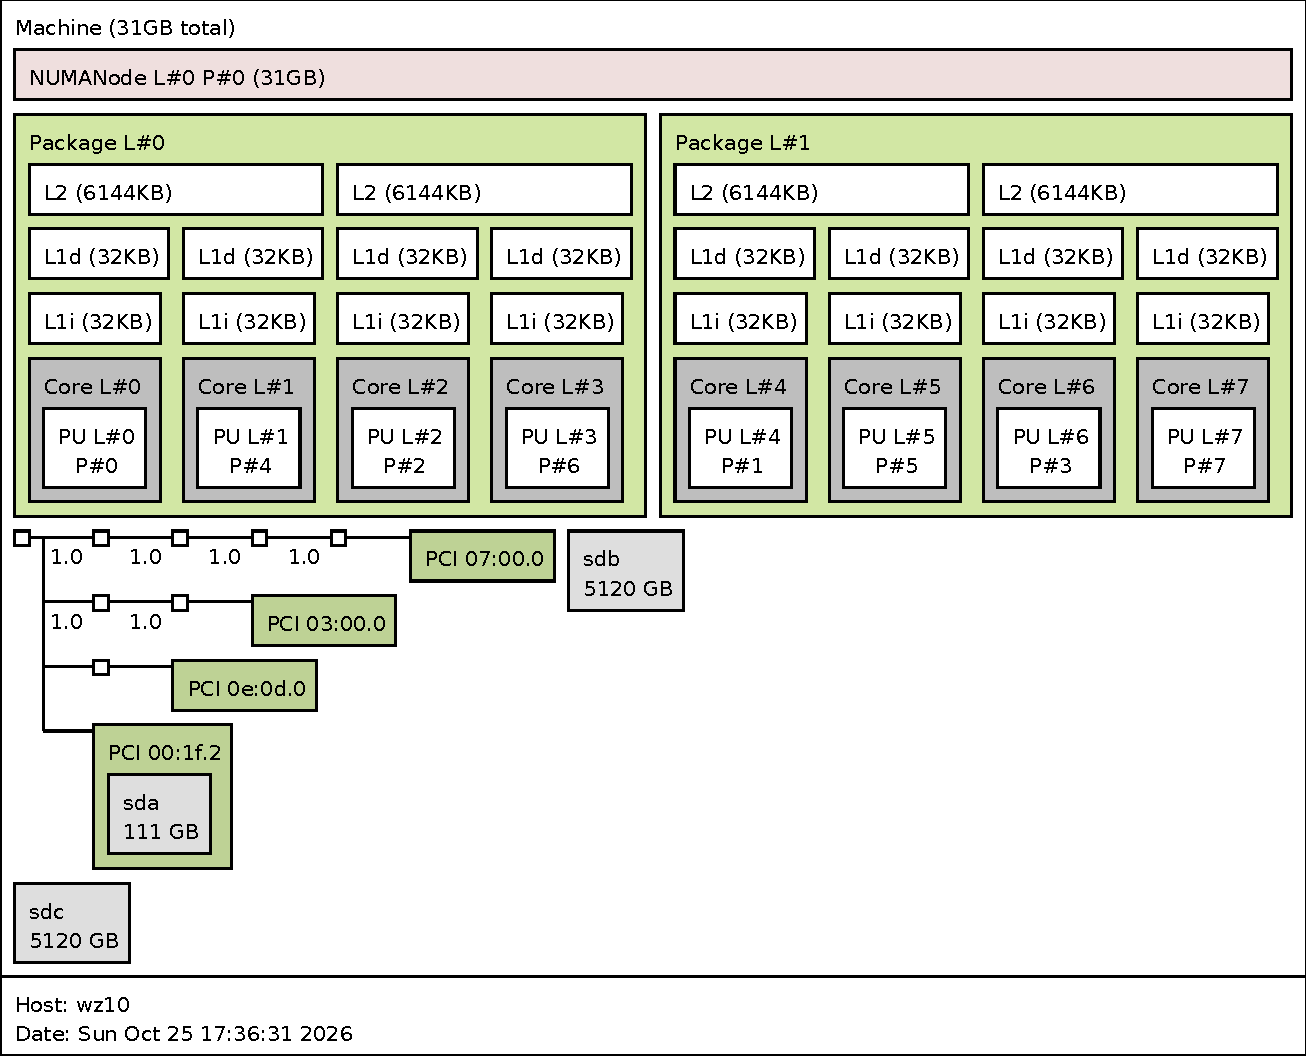
\includegraphics[width=0.88\textwidth]{topology.pdf}
    \label{fig:topology}
    \fonte{Gerado com o comando \texttt{lstopo} no cluster da disciplina.}
\end{figure}

% -----------------------------------------------------------------------------
\chapter{Metodologia Experimental e Escolha do Ladrilho}
% -----------------------------------------------------------------------------

\section{Escolha do Tamanho do Ladrilho ($w = 192$)}
Para definir o tamanho $w$ (\texttt{blockWidth}) do ladrilho na Versão B, levamos em conta duas coisas: ele precisava dividir exatamente o tamanho das matrizes em qualquer número de processos (1, 2, 3 ou 4) e os blocos precisavam caber com folga na cache L2 de $6\text{ MiB}$ ($6.144\text{ KiB}$):

\begin{enumerate}
    \item \textbf{Divisão Exata das Dimensões:} O valor $w = 192$ divide sem resto o número de colunas $M = 960$ ($5 \times 192$), $N_{cb} = 960$ ($5 \times 192$) e a quantidade de linhas $nl = N_{la} / nprocs$ de cada processo em todos os casos:
    \begin{itemize}
        \item $1\text{ processo}$: $nl = 2304 = 12 \times 192$;
        \item $2\text{ processos}$: $nl = 1152 = 6 \times 192$;
        \item $3\text{ processos}$: $nl = 768 = 4 \times 192$;
        \item $4\text{ processos}$: $nl = 576 = 3 \times 192$.
    \end{itemize}

    \item \textbf{Tamanho dos Blocos na Cache L2:} Cada ladrilho de $192 \times 192$ elementos do tipo \texttt{double} ($8\text{ bytes}$) ocupa:
    \begin{equation}
        \text{Tamanho de 1 Ladrilho} = 192 \times 192 \times 8\text{ bytes} = 294.912\text{ bytes} = 288\text{ KiB}
    \end{equation}
    Enquanto o código multiplica um bloco, ele precisa manter na cache 3 ladrilhos ao mesmo tempo (um de $A$, um de $B$ e um de $C$):
    \begin{equation}
        3\text{ Ladrilhos Ativos} = 3 \times 288\text{ KiB} = 864\text{ KiB} \approx 0,84\text{ MiB}
    \end{equation}
    Mesmo se contarmos uma linha inteira de 5 ladrilhos de $C$ ($5 \times 288\text{ KiB} = 1.440\text{ KiB}$) junto com 1 ladrilho de $A$ e 1 de $B$, o total dá $2.016\text{ KiB}$ ($\approx 1,97\text{ MiB}$), que é menos de um terço dos \textbf{$6\text{ MiB}$ ($6.144\text{ KiB}$)} da cache L2.
\end{enumerate}

\section{Medição dos Tempos de Computação e Comunicação}
No código, usamos dois cronômetros da biblioteca \nolinkurl{chrono.c}:
\begin{itemize}
    \item \textbf{Tempo Total ($T_{\text{total}}$):} Mede desde antes do \nolinkurl{MPI_Scatter} até o final do \nolinkurl{MPI_Gather}.
    \item \textbf{Tempo de Computação ($T_{\text{comp}}$):} Mede apenas a função que faz a multiplicação das matrizes localmente (\nolinkurl{mmul_kernel_versao_A} ou \nolinkurl{mmul_kernel_versao_B}).
    \item \textbf{Tempo de Comunicação ($T_{\text{comm}}$):} É a diferença $T_{\text{total}} - T_{\text{comp}}$, que corresponde ao tempo gasto trocando mensagens na rede (\nolinkurl{MPI_Scatter}, \nolinkurl{MPI_Bcast} e \nolinkurl{MPI_Gather}).
\end{itemize}

\section{Execução no Cluster e o Limite de 5 Minutos na Experiência A}
Nos scripts do SLURM (\nolinkurl{roda-exp-A-slurm.sh} e \nolinkurl{roda-exp-B-slurm.sh}), configuramos \textbf{10 execuções} para cada quantidade de processos ($1, 2, 3$ e $4$), totalizando 40 execuções por bateria:
\begin{itemize}
    \item \textbf{Experiência B (Versão B --- Blocada $w = 192$):} Como o cálculo com ladrilhos é muito rápido, as 40 execuções terminaram em apenas \textbf{$80\text{ segundos}$ ($1\text{ min }20\text{ s}$)} no Job 19391 (e repetimos no Job 19392 em $81\text{ s}$), rodando com muita folga.
    \item \textbf{Experiência A (Versão A --- Direta):} No Job 19390, conseguimos rodar todas as 40 execuções até o fim, e o script registrou um tempo total de \textbf{$303\text{ segundos}$ ($5\text{ min }03\text{ s}$)}.
\end{itemize}

\subsection{Por que a Experiência A rodou tudo em 5m03s na primeira vez e deu Timeout nas tentativas seguintes?}
Uma situação curiosa que aconteceu durante os nossos testes foi que o cluster cedido pelo professor tem um limite de tempo (\textit{timeout}) de \textbf{5 minutos ($300\text{ segundos}$)} por job. Quando submetemos a Experiência A com as nossas otimizações pela primeira vez (Job 19390), ela conseguiu rodar as 40 execuções completas marcando $5\text{ min }03\text{ s}$ ($303\text{ s}$). Porém, quando tentamos rodar o mesmo script novamente para fazer um segundo teste, o SLURM matou o job por \textit{timeout} antes de terminar.

Olhando os tempos gravados no arquivo \nolinkurl{saida-expA-job19390.txt}, dá para entender de forma bem simples por que isso aconteceu:
\begin{enumerate}
    \item \textbf{O tempo da Experiência A fica exatamente em cima dos 5 minutos:} Se somarmos apenas os tempos das 40 multiplicações que o programa imprimiu ($10 \times 12,54\text{ s}$ com 1 nó $+ 10 \times 6,65\text{ s}$ com 2 nós $+ 10 \times 4,52\text{ s}$ com 3 nós $+ 10 \times 3,49\text{ s}$ com 4 nós), já temos \textbf{$272\text{ segundos}$} só de conta. Porém, a cada uma das 40 execuções, o programa também precisa preencher as matrizes $A$ e $B$ com \texttt{rand()} fora do cronômetro, e nas 30 execuções com mais de 1 nó o comando \texttt{mpirun} precisa conectar nas outras máquinas (\texttt{wz10}, \texttt{wz11}, \texttt{wz12} e \texttt{wz15}) pela rede, criar os processos e depois encerrar tudo. Esse tempo extra fora do cronômetro gasta cerca de $0,7\text{ a }0,8\text{ s}$ por execução ($\approx 31\text{ s}$ nas 40 rodadas). Somando $272\text{ s} + 31\text{ s}$, o script leva justamente cerca de **$303\text{ segundos}$** para rodar.
    \item \textbf{Por que passou na primeira vez e caiu nas outras:} O SLURM não verifica o tempo dos jobs a cada milissegundo exato; ele checa de tempos em tempos (a cada alguns segundos) se algum job passou dos $300\text{ s}$. No Job 19390, a rede e as máquinas estavam livres naquele momento, então a última execução acabou aos $303\text{ s}$, bem nesse pequeno intervalo de poucos segundos antes do SLURM encerrar o job. Nas tentativas seguintes, qualquer pequena demora a mais na rede do laboratório para o \texttt{mpirun} iniciar os processos nas 4 máquinas (coisa de $3\text{ a }5\text{ segundos}$ a mais no total das 40 execuções) já fez o tempo passar de $306\text{--}308\text{ s}$, dando tempo do SLURM detectar que estourou os 5 minutos e cancelar o job na última bateria.
\end{enumerate}

% -----------------------------------------------------------------------------
\chapter{Resultados Experimentais e Análise de Desempenho}
% -----------------------------------------------------------------------------

Todos os valores medidos, médias e gráficos estão na planilha \nolinkurl{Planilha-MatMul-MPI-WZ-ExpA-ExpB.xlsx} e nos arquivos de saída dos Jobs 19390 e 19391 (e 19392).

\section{Experiência A --- Multiplicação Direta/Simples (Versão A)}
As Tabelas~\ref{tab:expA_tempos} e~\ref{tab:expA_gflops} mostram os tempos (Total, Computação e Comunicação), a vazão em GFLOPS e o Speedup das 10 execuções da Versão A para 1, 2, 3 e 4 processos MPI.

\begin{table}[htbp]
\centering
\caption{Tempos de Execução em Segundos (Total, Computação e Comunicação) — Experiência A (Versão A Direta, Job 19390).}
\label{tab:expA_tempos}
\resizebox{\textwidth}{!}{%
\begin{tabular}{lcccccccccccc}
\toprule
 & \multicolumn{3}{c}{\textbf{1 Proc (\texttt{wz10})}} & \multicolumn{3}{c}{\textbf{2 Procs (\texttt{wz10,11})}} & \multicolumn{3}{c}{\textbf{3 Procs (\texttt{wz10-12})}} & \multicolumn{3}{c}{\textbf{4 Procs (\texttt{wz10-12,15})}} \\
\cmidrule(lr){2-4} \cmidrule(lr){5-7} \cmidrule(lr){8-10} \cmidrule(lr){11-13}
\textbf{Execução} & \textbf{Total} & \textbf{Comp} & \textbf{Comm} & \textbf{Total} & \textbf{Comp} & \textbf{Comm} & \textbf{Total} & \textbf{Comp} & \textbf{Comm} & \textbf{Total} & \textbf{Comp} & \textbf{Comm} \\
\midrule
Execução 1 & 12,5682 & 12,5682 & 0,0000 & 6,7048 & 6,2429 & 0,4618 & 4,5011 & 4,1530 & 0,3482 & 3,4724 & 3,1424 & 0,3300 \\
Execução 2 & 12,5965 & 12,5965 & 0,0000 & 6,5949 & 6,2855 & 0,3094 & 4,5350 & 4,1623 & 0,3726 & \textbf{3,4574} & 3,1377 & 0,3197 \\
Execução 3 & 12,5218 & 12,5218 & 0,0000 & 6,6438 & 6,3025 & 0,3413 & 4,4871 & 4,1860 & 0,3011 & 3,5073 & 3,1611 & 0,3463 \\
Execução 4 & 12,5782 & 12,5782 & 0,0000 & 6,6479 & 6,3118 & 0,3361 & 4,4868 & 4,1483 & 0,3385 & 3,4988 & 3,1420 & 0,3568 \\
Execução 5 & 12,5930 & 12,5930 & 0,0000 & 6,7059 & 6,2576 & 0,4483 & 4,5566 & 4,1626 & 0,3940 & 3,4869 & 3,1434 & 0,3435 \\
Execução 6 & 12,5190 & 12,5190 & 0,0000 & 6,6266 & 6,2627 & 0,3639 & 4,5071 & 4,1781 & 0,3290 & 3,4660 & 3,1515 & 0,3145 \\
Execução 7 & 12,5121 & 12,5121 & 0,0000 & 6,7024 & 6,2667 & 0,4357 & 4,5659 & 4,1804 & 0,3854 & 3,4686 & 3,1389 & 0,3297 \\
Execução 8 & 12,4984 & 12,4984 & 0,0000 & 6,6069 & 6,2864 & 0,3205 & 4,5278 & 4,1514 & 0,3764 & 3,5483 & 3,1395 & 0,4088 \\
Execução 9 & 12,5660 & 12,5660 & 0,0000 & 6,6315 & 6,2769 & 0,3546 & 4,5288 & 4,2284 & 0,3004 & 3,4691 & 3,1434 & 0,3257 \\
Execução 10 & 12,4412 & 12,4412 & 0,0000 & 6,6241 & 6,2616 & 0,3625 & 4,5070 & 4,2160 & 0,2909 & 3,5675 & 3,1528 & 0,4147 \\
\midrule
\textbf{Média (s)} & \textbf{12,5394} & \textbf{12,5394} & \textbf{0,0000} & \textbf{6,6489} & \textbf{6,2755} & \textbf{0,3734} & \textbf{4,5203} & \textbf{4,1767} & \textbf{0,3437} & \textbf{3,4942} & \textbf{3,1453} & \textbf{0,3490} \\
Mínimo (s) & 12,4412 & 12,4412 & 0,0000 & 6,5949 & 6,2429 & 0,3094 & 4,4868 & 4,1483 & 0,2909 & 3,4574 & 3,1377 & 0,3145 \\
Máximo (s) & 12,5965 & 12,5965 & 0,0000 & 6,7059 & 6,3118 & 0,4618 & 4,5659 & 4,2284 & 0,3940 & 3,5675 & 3,1611 & 0,4147 \\
\textbf{\% Tempo} & \textbf{100,0\%} & \textbf{100,0\%} & \textbf{0,00\%} & \textbf{100,0\%} & \textbf{94,38\%} & \textbf{5,62\%} & \textbf{100,0\%} & \textbf{92,40\%} & \textbf{7,60\%} & \textbf{100,0\%} & \textbf{90,01\%} & \textbf{9,99\%} \\
\bottomrule
\end{tabular}%
}
\fonte{Dados extraídos de \nolinkurl{saida-expA-job19390.txt} nos nós \texttt{wz10}, \texttt{wz11}, \texttt{wz12} e \texttt{wz15}.}
\end{table}

\begin{table}[htbp]
\centering
\caption{Vazão em GFLOPS e Speedup Médio — Experiência A (Versão A Direta, Job 19390).}
\label{tab:expA_gflops}
\resizebox{\textwidth}{!}{%
\begin{tabular}{lcccc}
\toprule
\textbf{Execução} & \textbf{1 Proc (\texttt{wz10})} & \textbf{2 Procs (\texttt{wz10,11})} & \textbf{3 Procs (\texttt{wz10-12})} & \textbf{4 Procs (\texttt{wz10-12,15})} \\
\midrule
Execução 1 & 0,3379 & 0,6334 & 0,9435 & 1,2230 \\
Execução 2 & 0,3371 & \textbf{0,6439} & 0,9364 & \textbf{1,2283} \\
Execução 3 & 0,3391 & 0,6392 & 0,9464 & 1,2108 \\
Execução 4 & 0,3376 & 0,6388 & \textbf{0,9465} & 1,2138 \\
Execução 5 & 0,3372 & 0,6333 & 0,9320 & 1,2179 \\
Execução 6 & 0,3392 & 0,6409 & 0,9422 & 1,2252 \\
Execução 7 & 0,3394 & 0,6336 & 0,9301 & 1,2244 \\
Execução 8 & 0,3398 & 0,6428 & 0,9379 & 1,1968 \\
Execução 9 & 0,3380 & 0,6404 & 0,9377 & 1,2242 \\
Execução 10 & \textbf{0,3413} & 0,6411 & 0,9423 & 1,1904 \\
\midrule
\textbf{Média (GFLOPS)} & \textbf{0,3387} & \textbf{0,6387} & \textbf{0,9395} & \textbf{1,2155} \\
Mínimo (GFLOPS) & 0,3371 & 0,6333 & 0,9301 & 1,1904 \\
Máximo (GFLOPS) & 0,3413 & 0,6439 & 0,9465 & 1,2283 \\
\textbf{Speedup Total ($T_1/T_p$)} & \textbf{1,00$\times$} & \textbf{1,89$\times$} & \textbf{2,77$\times$} & \textbf{3,59$\times$} \\
\textbf{Speedup Computação} & \textbf{1,00$\times$} & \textbf{2,00$\times$} & \textbf{3,00$\times$} & \textbf{3,99$\times$} \\
\textbf{Eficiência Paralela} & \textbf{100,0\%} & \textbf{94,3\%} & \textbf{92,5\%} & \textbf{89,7\%} \\
\bottomrule
\end{tabular}%
}
\fonte{Dados extraídos de \nolinkurl{saida-expA-job19390.txt} nos nós \texttt{wz10}, \texttt{wz11}, \texttt{wz12} e \texttt{wz15}.}
\end{table}

\section{Experiência B --- Multiplicação Blocada com Ladrilhos ($w = 192$)}
As Tabelas~\ref{tab:expB_tempos} e~\ref{tab:expB_gflops} trazem os resultados das 10 execuções da Versão B com ladrilhos de $192 \times 192$ elementos (Job 19391).

\begin{table}[htbp]
\centering
\caption{Tempos de Execução em Segundos (Total, Computação e Comunicação) — Experiência B (Versão B Blocada, $w = 192$, Job 19391).}
\label{tab:expB_tempos}
\resizebox{\textwidth}{!}{%
\begin{tabular}{lcccccccccccc}
\toprule
 & \multicolumn{3}{c}{\textbf{1 Proc (\texttt{wz10})}} & \multicolumn{3}{c}{\textbf{2 Procs (\texttt{wz10,11})}} & \multicolumn{3}{c}{\textbf{3 Procs (\texttt{wz10-12})}} & \multicolumn{3}{c}{\textbf{4 Procs (\texttt{wz10-12,15})}} \\
\cmidrule(lr){2-4} \cmidrule(lr){5-7} \cmidrule(lr){8-10} \cmidrule(lr){11-13}
\textbf{Execução} & \textbf{Total} & \textbf{Comp} & \textbf{Comm} & \textbf{Total} & \textbf{Comp} & \textbf{Comm} & \textbf{Total} & \textbf{Comp} & \textbf{Comm} & \textbf{Total} & \textbf{Comp} & \textbf{Comm} \\
\midrule
Execução 1 & 1,9482 & 1,9482 & 0,0000 & 1,2221 & 0,9722 & 0,2499 & 0,9391 & 0,6485 & 0,2906 & 0,8013 & 0,4864 & 0,3149 \\
Execução 2 & 1,9478 & 1,9478 & 0,0000 & 1,2234 & 0,9727 & 0,2507 & 0,9420 & 0,6519 & 0,2901 & 0,8056 & 0,4863 & 0,3193 \\
Execução 3 & 1,9431 & 1,9431 & 0,0000 & 1,2224 & 0,9728 & 0,2496 & 0,9448 & 0,6525 & 0,2924 & 0,8019 & 0,4877 & 0,3142 \\
Execução 4 & 1,9473 & 1,9473 & 0,0000 & 1,2215 & 0,9728 & 0,2488 & 0,9475 & 0,6481 & 0,2994 & 0,8025 & 0,4874 & 0,3151 \\
Execução 5 & 1,9473 & 1,9473 & 0,0000 & 1,2212 & 0,9727 & 0,2485 & \textbf{0,9362} & 0,6486 & 0,2876 & \textbf{0,8002} & 0,4869 & 0,3133 \\
Execução 6 & 1,9463 & 1,9463 & 0,0000 & 1,2247 & 0,9778 & 0,2469 & 0,9366 & 0,6484 & 0,2881 & 0,8005 & 0,4866 & 0,3138 \\
Execução 7 & 1,9477 & 1,9477 & 0,0000 & 1,2251 & 0,9735 & 0,2516 & 0,9433 & 0,6532 & 0,2901 & 0,8039 & 0,4860 & 0,3180 \\
Execução 8 & 1,9516 & 1,9516 & 0,0000 & \textbf{1,2206} & 0,9738 & 0,2468 & 0,9849 & 0,6489 & 0,3359 & 0,8010 & 0,4859 & 0,3151 \\
Execução 9 & \textbf{1,9428} & 1,9428 & 0,0000 & 1,2215 & 0,9724 & 0,2492 & 0,9469 & 0,6481 & 0,2988 & 0,8027 & 0,4879 & 0,3148 \\
Execução 10 & 1,9437 & 1,9437 & 0,0000 & 1,2211 & 0,9729 & 0,2481 & 0,9455 & 0,6489 & 0,2966 & 0,8136 & 0,4858 & 0,3278 \\
\midrule
\textbf{Média (s)} & \textbf{1,9466} & \textbf{1,9466} & \textbf{0,0000} & \textbf{1,2224} & \textbf{0,9734} & \textbf{0,2490} & \textbf{0,9467} & \textbf{0,6497} & \textbf{0,2970} & \textbf{0,8033} & \textbf{0,4867} & \textbf{0,3166} \\
Mínimo (s) & 1,9428 & 1,9428 & 0,0000 & 1,2206 & 0,9722 & 0,2468 & 0,9362 & 0,6481 & 0,2876 & 0,8002 & 0,4858 & 0,3133 \\
Máximo (s) & 1,9516 & 1,9516 & 0,0000 & 1,2251 & 0,9778 & 0,2516 & 0,9849 & 0,6532 & 0,3359 & 0,8136 & 0,4879 & 0,3278 \\
\textbf{\% Tempo} & \textbf{100,0\%} & \textbf{100,0\%} & \textbf{0,00\%} & \textbf{100,0\%} & \textbf{79,63\%} & \textbf{20,37\%} & \textbf{100,0\%} & \textbf{68,63\%} & \textbf{31,37\%} & \textbf{100,0\%} & \textbf{60,59\%} & \textbf{39,41\%} \\
\bottomrule
\end{tabular}%
}
\fonte{Dados extraídos de \nolinkurl{saida-expB-w192-job19391.txt} nos nós \texttt{wz10}, \texttt{wz11}, \texttt{wz12} e \texttt{wz15}.}
\end{table}

\begin{table}[htbp]
\centering
\caption{Vazão em GFLOPS e Speedup Médio — Experiência B (Versão B Blocada, $w = 192$, Job 19391).}
\label{tab:expB_gflops}
\resizebox{\textwidth}{!}{%
\begin{tabular}{lcccc}
\toprule
\textbf{Execução} & \textbf{1 Proc (\texttt{wz10})} & \textbf{2 Procs (\texttt{wz10,11})} & \textbf{3 Procs (\texttt{wz10-12})} & \textbf{4 Procs (\texttt{wz10-12,15})} \\
\midrule
Execução 1 & 2,1798 & 3,4749 & 4,5221 & 5,3001 \\
Execução 2 & 2,1803 & 3,4713 & 4,5084 & 5,2714 \\
Execução 3 & 2,1855 & 3,4740 & 4,4947 & 5,2960 \\
Execução 4 & 2,1809 & 3,4766 & 4,4822 & 5,2919 \\
Execução 5 & 2,1808 & 3,4775 & \textbf{4,5360} & \textbf{5,3073} \\
Execução 6 & 2,1819 & 3,4677 & 4,5344 & 5,3053 \\
Execução 7 & 2,1804 & 3,4664 & 4,5019 & 5,2824 \\
Execução 8 & 2,1760 & \textbf{3,4791} & 4,3120 & 5,3015 \\
Execução 9 & \textbf{2,1859} & 3,4765 & 4,4847 & 5,2907 \\
Execução 10 & 2,1848 & 3,4779 & 4,4913 & 5,2200 \\
\midrule
\textbf{Média (GFLOPS)} & \textbf{2,1816} & \textbf{3,4742} & \textbf{4,4868} & \textbf{5,2866} \\
Mínimo (GFLOPS) & 2,1760 & 3,4664 & 4,3120 & 5,2200 \\
Máximo (GFLOPS) & 2,1859 & 3,4791 & 4,5360 & 5,3073 \\
\textbf{Speedup Total ($T_1/T_p$)} & \textbf{1,00$\times$} & \textbf{1,59$\times$} & \textbf{2,06$\times$} & \textbf{2,42$\times$} \\
\textbf{Speedup Computação} & \textbf{1,00$\times$} & \textbf{2,00$\times$} & \textbf{3,00$\times$} & \textbf{4,00$\times$} \\
\textbf{Eficiência Paralela} & \textbf{100,0\%} & \textbf{79,6\%} & \textbf{68,5\%} & \textbf{60,6\%} \\
\bottomrule
\end{tabular}%
}
\fonte{Dados extraídos de \nolinkurl{saida-expB-w192-job19391.txt} nos nós \texttt{wz10}, \texttt{wz11}, \texttt{wz12} e \texttt{wz15}.}
\end{table}

\section{Comparativo Direto: Experiência A vs. Experiência B}
A Tabela~\ref{tab:comparativo} resume a comparação direta entre a Versão A e a Versão B ($w = 192$).

\begin{table}[htbp]
\centering
\caption{Comparativo de Desempenho: Experiência A (Direta) vs. Experiência B (Blocada, $w = 192$).}
\label{tab:comparativo}
\resizebox{\textwidth}{!}{%
\begin{tabular}{cccccccccc}
\toprule
\textbf{Procs} & \textbf{Total A} & \textbf{Total B} & \textbf{Comp A} & \textbf{Comp B} & \textbf{Vazão A} & \textbf{Vazão B} & \textbf{Aceleração} & \textbf{Aceleração} & \textbf{Ganho Vazão} \\
\textbf{(Nós)} & \textbf{(s)} & \textbf{(s)} & \textbf{(s)} & \textbf{(s)} & \textbf{(GFLOPS)} & \textbf{(GFLOPS)} & \textbf{Total (A/B)} & \textbf{Comp (A/B)} & \textbf{\% (B vs A)} \\
\midrule
1 & 12,5394 & 1,9466 & 12,5394 & 1,9466 & 0,3387 & 2,1816 & \textbf{6,44$\times$} & \textbf{6,44$\times$} & \textbf{+544,04\%} \\
2 & 6,6489 & 1,2224 & 6,2755 & 0,9734 & 0,6387 & 3,4742 & \textbf{5,44$\times$} & \textbf{6,45$\times$} & \textbf{+443,92\%} \\
3 & 4,5203 & 0,9467 & 4,1767 & 0,6497 & 0,9395 & 4,4868 & \textbf{4,77$\times$} & \textbf{6,43$\times$} & \textbf{+377,56\%} \\
4 & 3,4942 & 0,8033 & 3,1453 & 0,4867 & 1,2155 & 5,2866 & \textbf{4,35$\times$} & \textbf{6,46$\times$} & \textbf{+334,94\%} \\
\bottomrule
\end{tabular}%
}
\fonte{Médias calculadas a partir dos Jobs SLURM 19390 e 19391.}
\end{table}

\section{Discussão dos Resultados}

\begin{enumerate}
    \item \textbf{Ganho de $6,45\times$ na Computação com Ladrilhos na Cache L2:} O resultado mais importante dos testes é a queda drástica no tempo de cálculo da Versão B ($w = 192$) em relação à Versão A. Com 1 processo, o tempo caiu de $12,5394\text{ s}$ para $1,9466\text{ s}$ (\textbf{6,44 vezes mais rápido}, ou $+544,04\%$ de vazão). Com 2, 3 e 4 processos, o ganho no tempo de computação continuou praticamente o mesmo, entre \textbf{$6,43\times$ e $6,46\times$}. Isso mostra na prática a diferença que faz manter os três blocos de $288\text{ KiB}$ ($864\text{ KiB}$ no total) dentro da cache L2 de $6\text{ MiB}$ e percorrer as linhas de $B$ e $C$ sequencialmente (passo 1), em vez de ficar dando saltos de $960$ elementos pelas colunas de $B$ como na Versão A.

    \item \textbf{Divisão Linear do Tempo de Computação entre os Nós:} Olhando apenas para o tempo gasto calculando ($T_{\text{comp}}$), o trabalho escalou de forma linear ao adicionar mais nós:
    \begin{itemize}
        \item Na \textbf{Versão A}, o tempo de computação caiu de $12,5394\text{ s}$ (1 nó) para $6,2755\text{ s}$ (2 nós, $2,00\times$), $4,1767\text{ s}$ (3 nós, $3,00\times$) e $3,1453\text{ s}$ (4 nós, \textbf{$3,99\times$}).
        \item Na \textbf{Versão B}, o tempo de computação caiu de $1,9466\text{ s}$ (1 nó) para $0,9734\text{ s}$ (2 nós, $2,00\times$), $0,6497\text{ s}$ (3 nós, $3,00\times$) e $0,4867\text{ s}$ (4 nós, \textbf{$4,00\times$}).
    \end{itemize}
    Isso acontece porque cada nó recebe uma fração exata das linhas ($N_{la}/nprocs$) e faz a sua parte da conta sem precisar trocar mensagens durante o cálculo.

    \item \textbf{Impacto do Tempo de Rede (Comunicação MPI):} O tempo gasto enviando e recebendo as matrizes pela rede Ethernet ($T_{\text{comm}}$) ficou parecido nas duas versões (em torno de $0,25\text{ s}$ a $0,37\text{ s}$), já que a quantidade de bytes transmitidos no \nolinkurl{MPI_Scatter}, \nolinkurl{MPI_Bcast} e \nolinkurl{MPI_Gather} é a mesma. Porém, como a Versão B faz a conta muito mais rápido ($0,4867\text{ s}$ em 4 nós contra $3,1453\text{ s}$ na Versão A), o tempo de rede acaba pesando bem mais na Versão B: em 4 nós, a comunicação representa apenas \textbf{$9,99\%$} do tempo total na Versão A, mas chega a \textbf{$39,41\%$} do tempo total na Versão B. Por isso o Speedup Total da Versão B em 4 nós fica em $2,42\times$ (contra $3,59\times$ na Versão A), mesmo a Versão B entregando uma vazão final muito maior ($5,2866\text{ GFLOPS}$ contra $1,2155\text{ GFLOPS}$).
\end{enumerate}

% -----------------------------------------------------------------------------
\chapter{Instruções de Compilação, Execução e Arquivos Entregues}
% -----------------------------------------------------------------------------

\section{Como Compilar o Projeto}
O projeto inclui um \texttt{Makefile} que compila o código usando \texttt{mpicc} com as flags \texttt{-Wall -Wextra -O3 -march=native -funroll-loops -std=gnu11}:
\begin{verbatim}
make clean && make
\end{verbatim}
Isso gera o executável \texttt{mmul}, que serve tanto para a Versão A quanto para a Versão B.

\section{Como Executar o Programa}
O programa recebe as dimensões das matrizes e as flags opcionais pela linha de comando:
\begin{itemize}
    \item \textbf{Versão A (Direta/Simples):}
    \begin{verbatim}
    mpirun -np <n> ./mmul <Nla> <M> <Ncb> [-v]
    \end{verbatim}
    Exemplo: \texttt{mpirun -np 4 ./mmul 2304 960 960 -v}
    \item \textbf{Versão B (Blocada com Ladrilhos):}
    \begin{verbatim}
    mpirun -np <n> ./mmul <Nla> <M> <Ncb> -w <blockWidth> [-v]
    \end{verbatim}
    Exemplo: \texttt{mpirun -np 4 ./mmul 2304 960 960 -w 192 -v}
\end{itemize}
Se a opção \texttt{-v} for passada, o processo 0 roda a função \nolinkurl{verifica_resultado} ao final e avisa se todos os elementos bateram com a multiplicação sequencial.

\section{Como Submeter os Experimentos no SLURM}
No cluster da disciplina, os experimentos são colocados na fila com:
\begin{verbatim}
sbatch roda-exp-A-slurm.sh
sbatch roda-exp-B-slurm.sh
\end{verbatim}

\section{Estrutura dos Arquivos Entregues}
O arquivo compactado da entrega contém:

\begin{itemize}
    \item \textbf{Códigos-Fonte em C e Cabeçalhos:}
    \begin{itemize}
        \item \nolinkurl{mmul.c} e \nolinkurl{mmul.h}: código principal em MPI (Versão A e Versão B), geração das matrizes (\nolinkurl{gera_matriz}) e conferência do resultado (\nolinkurl{verifica_resultado});
        \item \nolinkurl{chrono.c} e \nolinkurl{chrono.h}: funções de medição de tempo.
    \end{itemize}

    \item \textbf{Scripts de Compilação, Teste e SLURM:}
    \begin{itemize}
        \item \nolinkurl{Makefile}: compilação com \texttt{mpicc};
        \item \nolinkurl{roda-exp-A-slurm.sh}: script SLURM da Experiência A (10 execuções para 1 a 4 processos);
        \item \nolinkurl{roda-exp-B-slurm.sh}: script SLURM da Experiência B com $w = 192$ (10 execuções para 1 a 4 processos);
        \item \nolinkurl{roda-verifica.sh}: script para testar a corretude com a flag \texttt{-v};
        \item \nolinkurl{coleta-hardware.sh}: script para coletar dados do processador (\texttt{lscpu} e \texttt{lstopo}).
    \end{itemize}

    \item \textbf{Planilha e Saídas do Cluster:}
    \begin{itemize}
        \item \nolinkurl{Planilha-MatMul-MPI-WZ-ExpA-ExpB.xlsx}: planilha com 4 abas (\texttt{Exp A - Direta}, \texttt{Exp B - Blocada w=192}, \texttt{Comparativo A vs B} e \texttt{Hardware e SLURM}), fórmulas e 6 gráficos;
        \item \nolinkurl{saida-expA-job19390.txt} e \nolinkurl{resultados-expA-direta-job19390.txt}: saídas completas da Experiência A;
        \item \nolinkurl{saida-expB-w192-job19391.txt}, \nolinkurl{resultados-expB-blocada-job19391.txt}, \nolinkurl{saida-expB-w192-job19392.txt} e \nolinkurl{resultados-expB-blocada-job19392.txt}: saídas completas da Experiência B;
        \item \nolinkurl{teste-local.txt}, \nolinkurl{lscpu.txt} e \nolinkurl{lstopo.txt}: arquivos de teste e informações de hardware.
    \end{itemize}

    \item \textbf{Relatório, Topologia e Especificação Original:}
    \begin{itemize}
        \item \nolinkurl{relatorio.pdf}: relatório em PDF (e o código-fonte LaTeX em \nolinkurl{Relatorio_LaTeX_UFPR.zip});
        \item \nolinkurl{topology.pdf} e \nolinkurl{topology.svg}: figuras da topologia geradas pelo \texttt{lstopo};
        \item \nolinkurl{trab2-matmul-MPI-pp-2sem26.pdf} e \nolinkurl{trab2-mmul-blocada-com-ladrilhos.pdf}: PDFs originais da especificação.
    \end{itemize}
\end{itemize}

% -----------------------------------------------------------------------------
\chapter{Conclusão}
% -----------------------------------------------------------------------------

Com este trabalho foi possível ver na prática como o paralelismo entre várias máquinas com MPI se combina com a otimização de memória cache dentro de cada processador.

A divisão das matrizes $A$ e $C$ em faixas horizontais (\nolinkurl{MPI_Scatter} e \nolinkurl{MPI_Gather}) junto com o envio de $B$ (\nolinkurl{MPI_Bcast}) dividiu bem o peso da conta entre os 4 nós do cluster (\texttt{wz10}, \texttt{wz11}, \texttt{wz12} e \texttt{wz15}), alcançando um Speedup de computação de $3,99\times$ na Versão A e $4,00\times$ na Versão B com 4 nós.

Ao mesmo tempo, a comparação entre as duas versões mostrou que apenas dividir o trabalho na rede não basta se o acesso à memória local for ruim: ao usar ladrilhos de $192 \times 192$ elementos ($288\text{ KiB}$ por bloco) que cabem na cache L2 de $6\text{ MiB}$ e trocar a ordem dos laços internos para $i \to k \to j$, a Versão B calculou as mesmas matrizes cerca de $6,45\times$ mais rápido que a Versão A, subindo a vazão média em 4 nós de $1,2155\text{ GFLOPS}$ para $5,2866\text{ GFLOPS}$ (e fazendo a bateria completa de 40 execuções no cluster cair de $303\text{ segundos}$ para apenas $80\text{ segundos}$).

\postextual

% -----------------------------------------------------------------------------
\begin{apendicesenv}
\partapendices

\chapter{Saída Completa do Comando \texttt{lscpu} nos Nós do Cluster}
\label{apendice:lscpu}

Registro obtido nos nós de computação \texttt{wz10}--\texttt{wz15} (Intel Xeon E5410 @ 2.33GHz):

\begin{lstlisting}[breaklines=true, basicstyle=\ttfamily\scriptsize]
Architecture:                    x86_64
CPU op-mode(s):                  32-bit, 64-bit
Byte Order:                      Little Endian
Address sizes:                   38 bits physical, 48 bits virtual
CPU(s):                          8
On-line CPU(s) list:             0-7
Thread(s) per core:              1
Core(s) per socket:              4
Socket(s):                       2
NUMA node(s):                    1
Vendor ID:                       GenuineIntel
CPU family:                      6
Model:                           23
Model name:                      Intel(R) Xeon(R) CPU           E5410  @ 2.33GHz
Stepping:                        10
CPU MHz:                         2333.000
CPU max MHz:                     2333.0000
CPU min MHz:                     2000.0000
BogoMIPS:                        4655.52
Virtualization:                  VT-x
L1d cache:                       256 KiB
L1i cache:                       256 KiB
L2 cache:                        24 MiB
NUMA node0 CPU(s):               0-7
Vulnerability Itlb multihit:     KVM: Mitigation: VMX disabled
Vulnerability L1tf:              Mitigation; PTE Inversion; VMX EPT disabled
Vulnerability Mds:               Vulnerable: Clear CPU buffers attempted, no microcode; SMT disabled
Vulnerability Meltdown:          Mitigation; PTI
Vulnerability Spec store bypass: Vulnerable
Vulnerability Spectre v1:        Mitigation; usercopy/swapgs barriers and __user pointer sanitization
Vulnerability Spectre v2:        Mitigation; Full generic retpoline, STIBP disabled, RSB filling
Vulnerability Srbds:             Not affected
Vulnerability Tsx async abort:   Not affected
Flags:                           fpu vme de pse tsc msr pae mce cx8 apic sep mtrr pge mca cmov pat pse36 clflush dts acpi mmx fxsr sse sse2 ht tm pbe syscall nx lm constant_tsc arch_perfmon pebs bts rep_good nopl cpuid aperfmperf pni dtes64 monitor ds_cpl vmx est tm2 ssse3 cx16 xtpr pdcm dca sse4_1 xsave lahf_lm pti tpr_shadow vnmi flexpriority vpid dtherm
\end{lstlisting}

\end{apendicesenv}

\end{document}
